\section{Recasting Inside the Experimental Collaborations}
\label{sec:ch5-recastingInsideExp}

Reinterpretations performed within the experiments themselves present unique advantages and disadvantages. They allow for thorough and consistent treatment of detector effects and geometry, object reconstruction, and systematic uncertainties in a way which is impossible through external recasting. Groups can share resources and easily communicate all necessary details. On the other hand, they are of course limited to the model(s) chosen for reinterpretation. In the ideal situation, reinterpretation(s) which provide meaningful results can be performed with minimal overhead to a given analysis.

As the LHC enters an era of decelerating luminosity growth and following larger trends in analysis techniques, the LHC analyses become harder to re-implement with sufficient accuracy outside of the experiments compared to cut-based analyses. Increasingly analysis utilize machine learning algorithms that transform a large number of event-level and particle-level observables into higher-level discriminants, which are not easily characterized by low-dimensional efficiency tables and may require inputs that third-party detector simulations are not able to re-produce. In particular non-prompt searches may depend on non-traditional reconstruction objects and details of the detector simulation and geometry in ways that require a more detailed simulation than is achievable by e.g. third-party simulators. Hence, experiments are investigating approaches that enable internal re-interpretation using the full set of available information.

Full-fidelity reinterpretations are also especially relevant for long-lived particles, since the signal simulation may depend more heavily on details not well captured by third-party simulation tools. For example, for sufficiently high lifetime, the decays must be handled by a full detector simulation such as GEANT (or some complex interaction between GEANT and Monte-Carlo packages such as Pythia). Such decays are not well-covered by tools like Delphes as the response of such in-detector decays may require access to a more detailed geometry description.

\subsection{The RECAST Framework}

The RECAST Framework~\cite{Cranmer2011} is a developing platform for experiments as well as authors of non-experiment re-implementations of LHC analyses that enables cloud-based analysis execution and common presentation of reinterpretation results. The framework consists of two components

\paragraph{The RECAST frontend:} a web-based service, where reinterpretation of analyses can be suggested by interested authors that provide necessary inputs such as UFO model files, process and parameter card templates, or suggested scan grids. Responses to such requests, possibly by more than one analysis implementation, can then be uploaded. Such a web-service, interfaced with services such as HepData may then serve as a resource for the LHC community to organize and share reinterpretation results obtained by the various analysis implementations.

\paragraph{The RECAST backend:} An important objective of the framework is to enable a full-fidelity re-interpretation using the original analysis code developed within the experiment that is approvable by the collaboration and on an equal footing with the original publication. In contrast to third-party recastng tools, in which multiple analyses are implemented using a single, common framework, which can executed on a single computing element, such an exact analysis re-execution often necessitates a distributed data analysis using a number different frameworks in use within the experiments. Therefore RECAST has developed a flexible graph-based, analysis description and execution backend[cite ACAT 2017] that enables a faithful re-execution of nearly arbitrary analysis code on cloud platforms such as those offered by CERN~\footnote{Thanks to this flexibility, the popular third party recasting tools can easily be integrated into this backend as well, with current integrations being available for CheckMate and Rivet.}. The backend provides experiments with an access-controlled interface to view reinterpretation requests, retrieve the necessary analysis description from repositories such as the CERN Analysis Preservation Portal (CAP)~\cite{CAP},  execute the analysis on datasets for the new model and -- if approved -- upload the results to the public frontend. Figure~\ref{fig:recast-cc} shows a screenshot of the current prototype user interface, giving collaboration members an overview over requested points as well as controls to steer processing and submission.

These services are being developed in close collaboration with the CERN Analysis Preservation project, which is a common project supported by the four major LHC experiments. While this integration work is on-going, the computing backend for RECAST has been successfully used for a number of Run-1 and Run-2 re-interpretations published by the ATLAS Experiment.


\subsection{Analysis Preservation as a driver for re-interpretation}

Within the LHC experiments, the ability to re-interpret analyses is, perhaps unintuitively, mostly limited by the internal availability of the analysis routines for a given to the wider collaboration as opposed to e.g. availability of computing resource constraints. The large number of measurements and searches, the heterogeneity and complexity of the analysis software, as well the size of the collaboration lead to a situation in which oftentimes only a small number of analyzers of the original analysis team is able to execute any given analysis. Furthermore, due to the collaborative development model, analyzers typically are responsible for only a subset of the analysis resulting in knowledge fragmentation. Therefore both ATLAS and CMS are now designing interface to store analysis-relevant information CERN Analysis Preservation Portal~\cite{CAP} to mitigate this problem. In the context of RECAST the software and analysis-workflow preservation aspects of this effort are most relevant. The former is mainly implemented through archiving of source code repositories and the archival Linux Containers, which now enjoy wide-spread industry support, while internal structure of the analysis workflow is archived in CAP in the form of declarative workflow specifications such as yadage~\cite{Cranmer:2017frf}, which has been developed for RECAST, and the Common Workflow Language (CWL)\cite{CWL}. It is planned that CAP and RECAST will utilize a common computing backend in order to re-execute the analyses that have been preserved in the portal. As the preservation is enabled by recent technological advances and the process of archival is increasingly streamlined, it is expected that a higher number of  experiment-internal analysis codes will be available for RECAST.

\begin{figure}[h]
\begin{center}
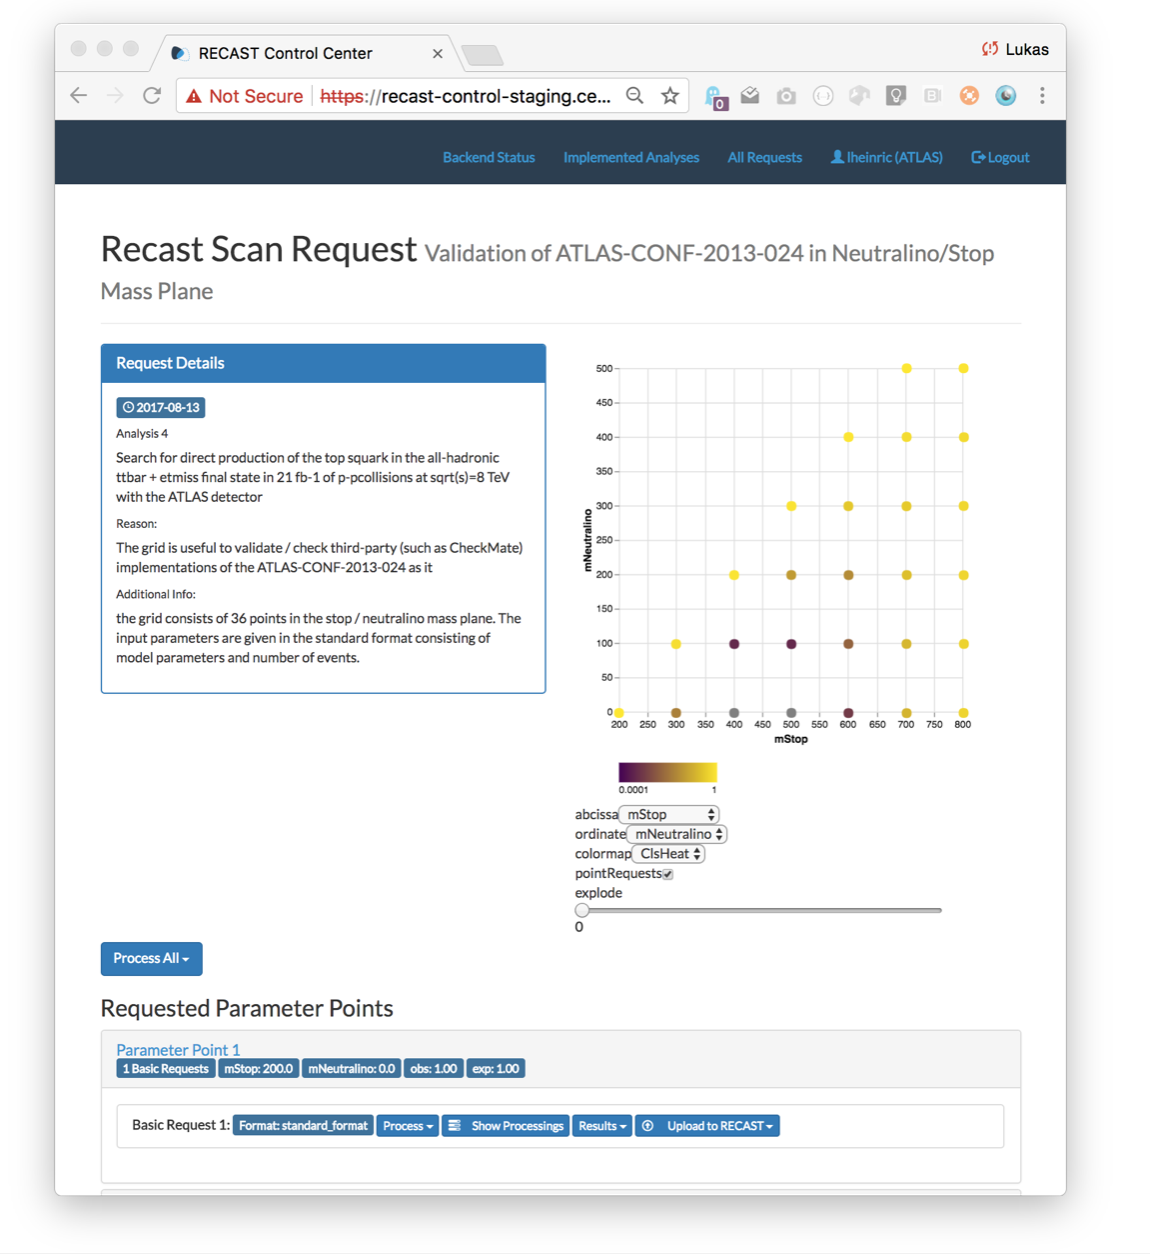
\includegraphics[width=0.5\textwidth,angle=0]{ch5-figures/requestview.png}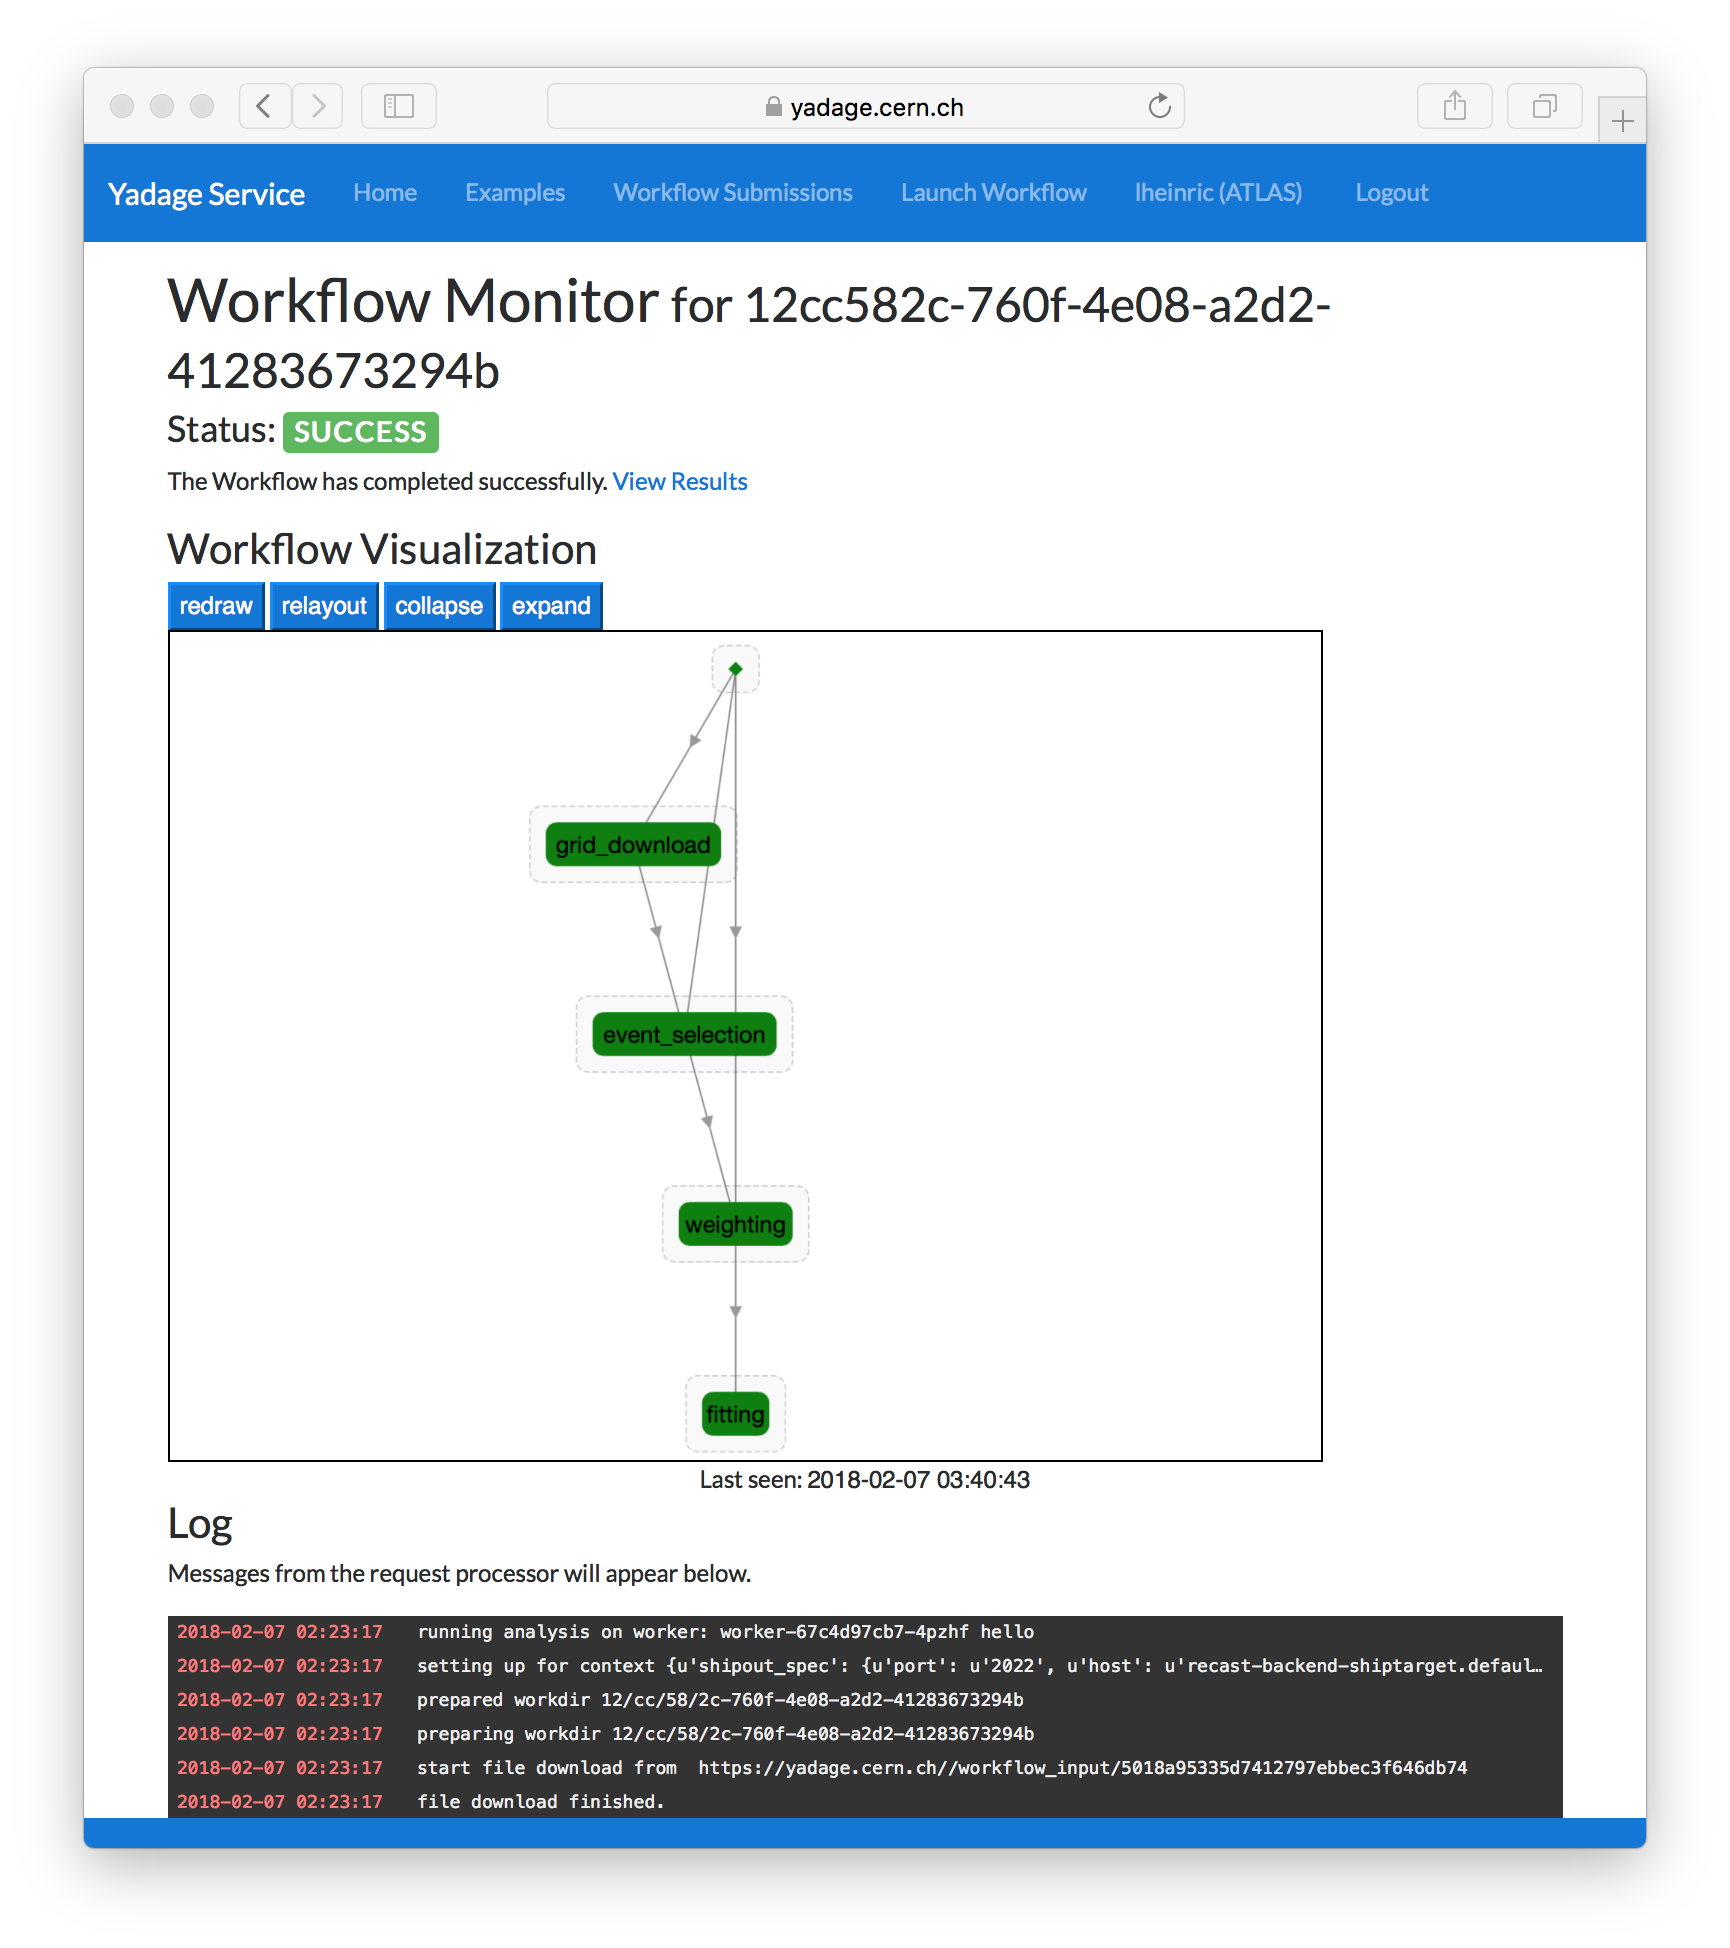
\includegraphics[width=0.5\textwidth,angle=0]{ch5-figures/monitor.png}

\end{center}
\caption{
Left: Web-based interface for RECAST backend for experiment that presents the requested parameter points and color-coded results,
Right: An experiment-internal reinterpretation executing on the distributed infrastructure built by CAP and RECAST.}
\label{fig:recast-cc}
\end{figure}

\subsection{RECAST Examples}

\subsubsection{ATLAS-internal Analysis Examples and Results}

A number of re-interpretation publications have been supported by the backend underpinning RECAST. After Run-1, ATLAS has conducted a thorough re-interpretation of the SUSY landscape in the context of the phenomenological pMSSM~\cite{Aad:2015baa}, a study involving 20 SUSY analyses and 50,000 fully simulated pMSSM parameter points. While at that time, most analyses had to be re-interpreted manually, the 2L electroweak analysis~\cite{Aad:2014vma} included in that paper served as a protootype analysis and provided results using the highly automated RECAST backends.

The analysis was than later re-used with minimal additional effort in two additional publications that focused on more domain-specific SUSY realizations: a five-dimensional dark-matter reinterpretation of electroweak seaches~\cite{Aaboud:2016wna}, as well as a reinterpretations in the context of general gauge-mediated models~\cite{ATLAS-CONF-2016-033}.

\begin{figure}[h]
\begin{center}
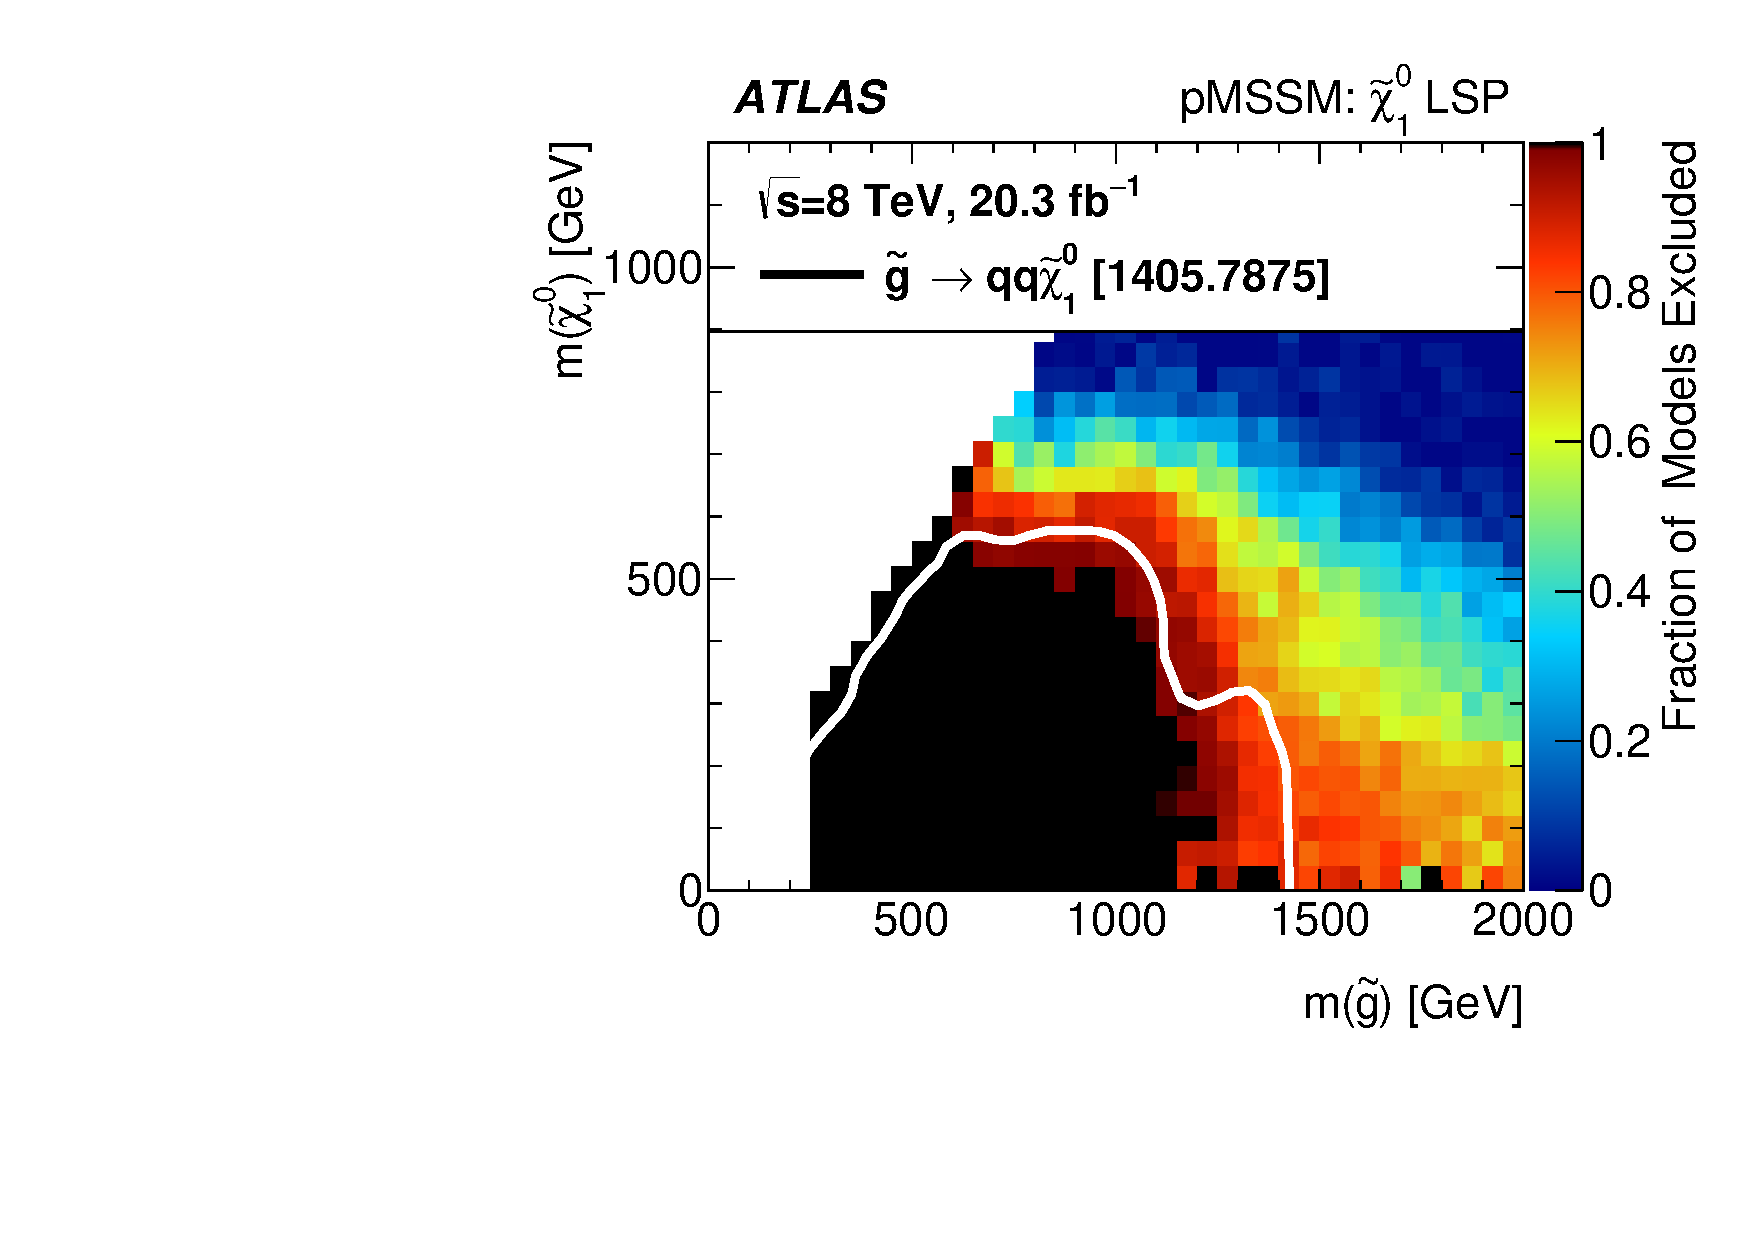
\includegraphics[width=0.5\textwidth,angle=0]{ch5-figures/pMSSM.pdf}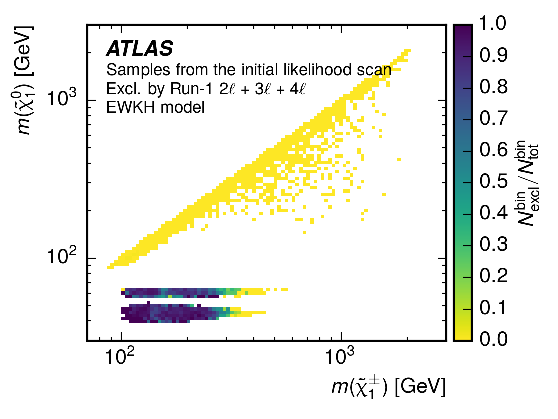
\includegraphics[width=0.5\textwidth,angle=0]{ch5-figures/DM.pdf}

\end{center}
\caption{
Left: pMSSM exclusion in the gluino-neutralino mass-plane. Results partially provided by RECAST.
Right: Follow-up dark-matter re-interpretation. Exclusions presented in chargino-neutralino mass-plane.
}
\label{fig:recast-cc}
\end{figure}

[We have a nother reinterpretation of a multi-bjet Run-2 analysis in the pipline for Moriond. Depending on timelines, I would love to include this]

Currently, a number of additional Run-2 analyses are in the process of being re-interpreted with results expected to appear soon.

\subsubsection{Third-Party Tool Integration}

Both the CheckMate and the Rivet analysis catalogues have been implemented in the analysis execution framework. Both are configured to analyze events that are provided in the HepMC format. Due to the modular approach of the analysis backend, a number of Monte Carlo generation workflows, such as Herwig, SHERPA or Madgraph, can be used depending on their ability to correctly model the desired signal.

For analyses, where multiple implementation exists: e.g. from multiple third-party tools such as Rivet BSM, CheckMate or MadAnalysis as well as from multiple experiment-internal configurations (fast Simulation, full simulation), RECAST will allow the community to compare and contrast of reinterpretation results.

\subsubsection{Outlook}

Thanks to industry-backed technological advances, a realistic technical solution to the Analysis Preservation problem for the LHC experiments and the original RECAST proposal has come into view. The initial use of such infrastructure for the reinterpretation for prompt SUSY searches is generalized easily for long-lived particle searches as the tools used for both signal simulation and analysis preservaton and execution do not make simplifying assumption on the nature of the BSM signal or analysis structure.  As such, RECAST may cover reinterpretation use-cases, where either third-party reinterpretations are impossible due to missing public information or limitations of third-party tools or accurate, experiment-approved results are desired.
